% \documentclass{report}
% \begin{document}
\subsection{Fonctionnement du client GUI}
Le client GUI peut recevoir en paramètre l'ip ou le nom de domaine du serveur auquel il doit se connecter, mais c'est facultatif, il le demandera a l'utilisateur si on ne lui donne pas. Une fois connecté au serveur, le client affichera la liste des films dans l'ordre de la base de données, on pourra alors se connecter à un compte, s'inscrire, avoir des recommendations personnalisées, voir les tendances, etc....\par
Le client utilise le moteur de rendu Webkit pour afficher l'interface, le code HTML donné au moteur est généré en interne par le client. Les liens cliquables sont interceptés, les requêtes web sont annulées, et remplacées par une execution de code local. Les seules véritables requêtes HTTP réalisées sur l'interfaces sont celles permettant d'afficher le lecteur youtube.\par
Les pages \og web \fg de l'interface sont réalisées a partir de fichiers json. exec://main.json va demander au client de charger le fichier se trouvant dans: web/main.json. Ce fichier sera interprété par un générateur de code HTML maison qui génère l'intégralité de l'interface en se basant sur ce qui est présent dans le json. Les fichiers json permettent d'ajouter des fichiers css, des fichiers de scripts, des tags HTML, inclure des fichiers, ou appeler des fonctions C.\par
La majorité du code de l'interface est généré via des fonctions C, chaque fonction à la même signature, ce qui permet de faire une hashmap de pointeurs de fonction qui associe un nom à une fonction. Le nom est entré dans le json, ce qui permet a l'interface de choisir la bonne fonction, et les paramètres sont passés a la fonction depuis le fichier JSON. Il est possible de faire des appels récursifs de fonctions, par exemple, le lecteur youtube peut être appelé depuis un fichier JSON pour afficher une vidéo, mais il peut aussi être appellé depuis une autre fonction du générateur pour l'intégrer facilement dans la mise en page.\par

\begin{figure}[H]
	\begin{center}
		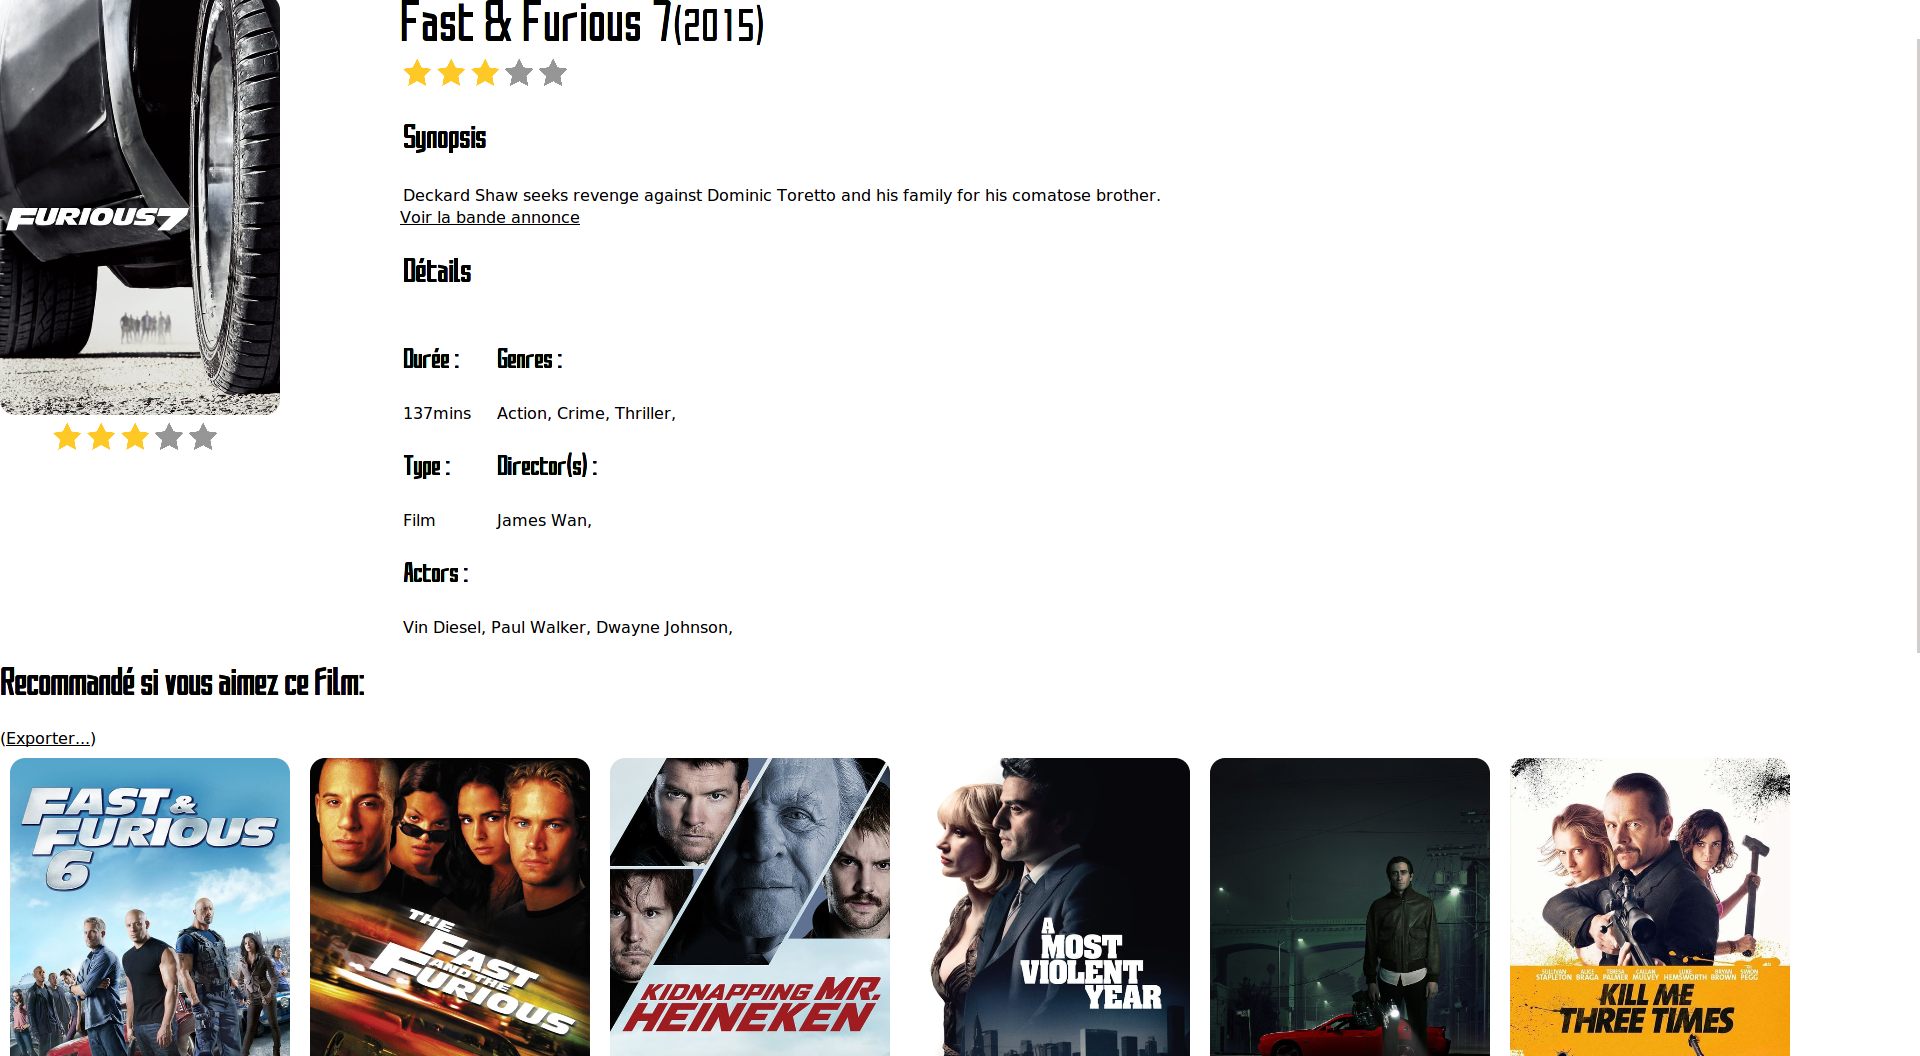
\includegraphics[scale=0.20]{img/film_gui.png}
	\end{center}
	\caption{Interface graphique de la page du film Fast \& Furious 7}
\end{figure}

Les interactions directes avec un utilisateur, liens cliquables, formulaires et redirections sont assurées par la transmission dans l'URL de la requête à l'interface, ces paramètres sont extraits par le générateur HTML, et sont transmis par un Vector\_t (tableau dynamique de chaines de caractères) aux fonctions permettant d'obtenir le code final qui sera executé par Webkit.\par
Une certain nombre de fonctions de Webkit ont été modifiées et/ou désactivées pour que l'interface ne puisse être utilisée que dans le cadre du projet, et non pas pour surfer n'importe où sur internet, ces modifications nous ont permis d'obtenir une interface stable et dans l'ère du temps.\par
% \end{document}


\begin{figure}[H]
	\begin{center}
		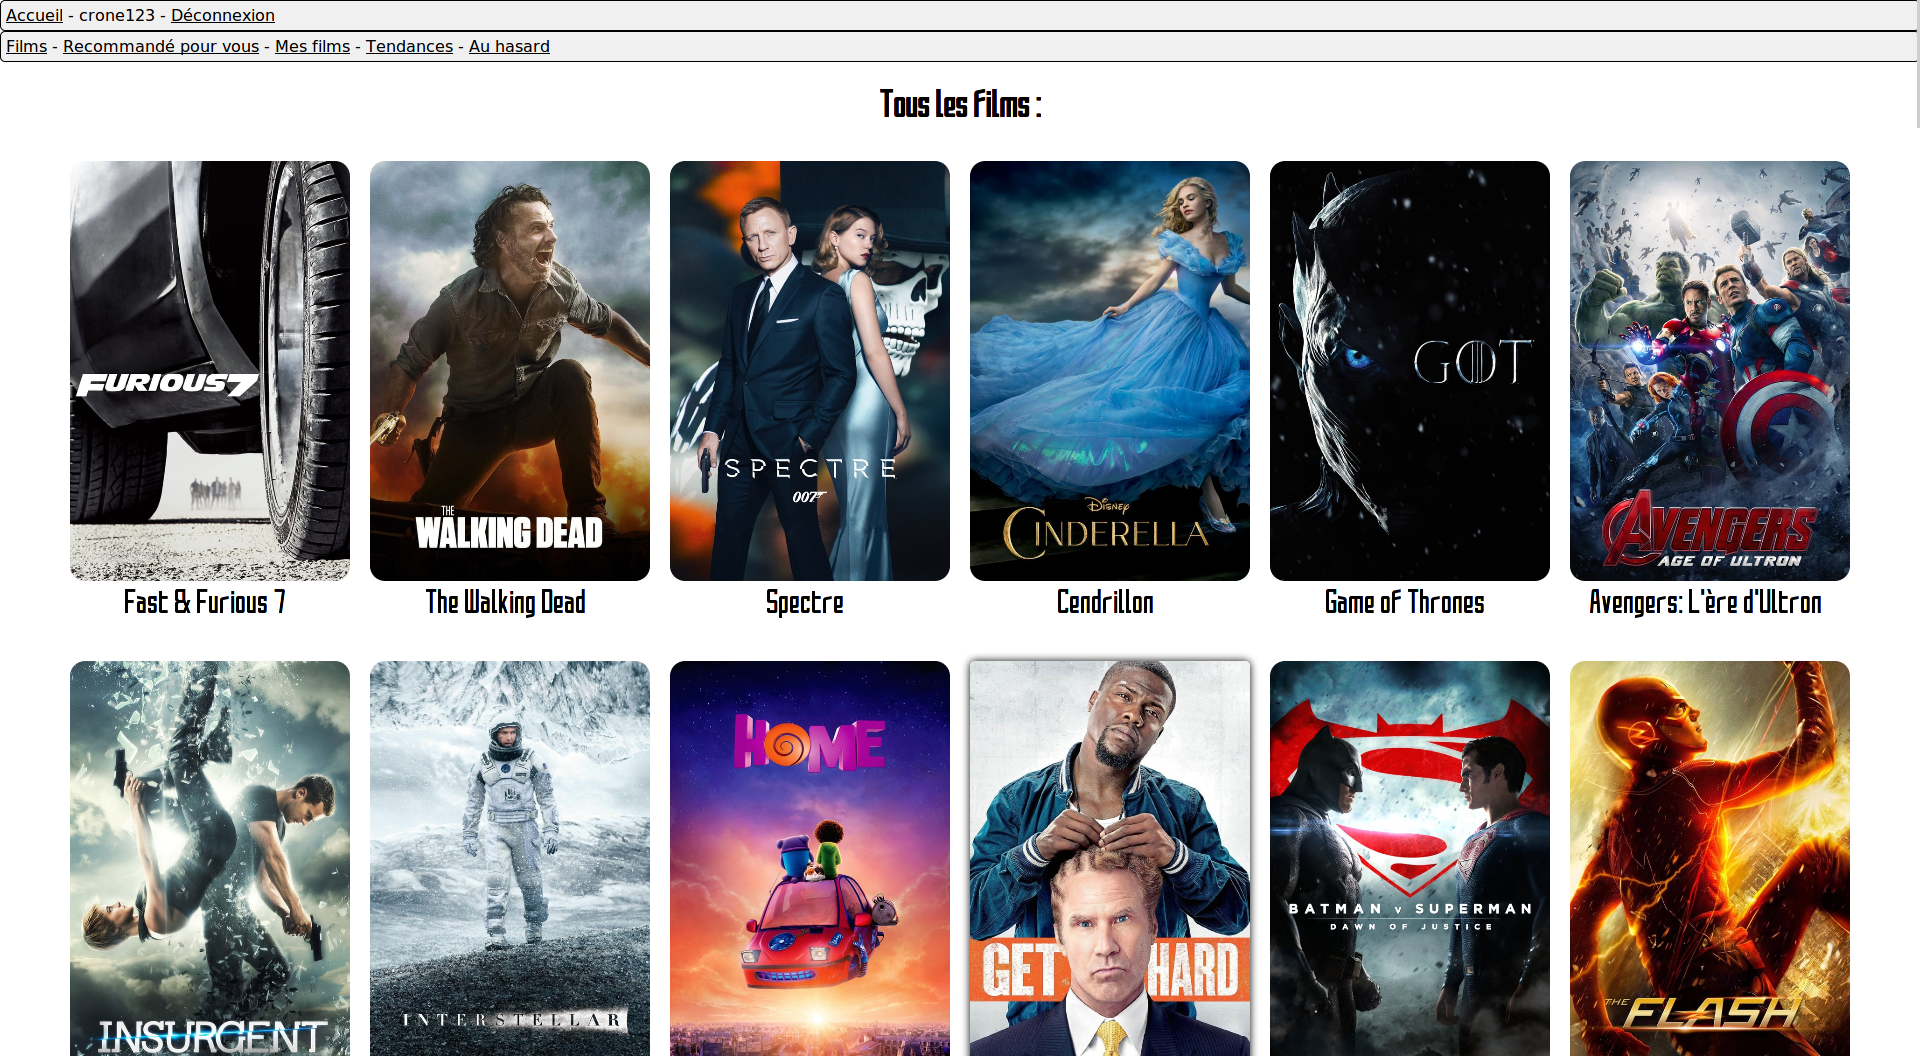
\includegraphics[scale=0.20]{img/films_gui.png}
	\end{center}
	\caption{Interface graphique du menu films}
\end{figure}
